\documentclass[tikz,border=8pt]{standalone}
% Shared look for every TikZ diagram. Load with \input{../../tools/tikz-style.tex}
\usepackage[T1]{fontenc}
\usepackage{lmodern}
\renewcommand{\sfdefault}{lmr}  % diagrams use the same serif as the text
\usetikzlibrary{arrows.meta, positioning, shapes.geometric, calc, fit, backgrounds}
\definecolor{cblue}{HTML}{4C78A8}
\definecolor{corange}{HTML}{F58518}
\definecolor{cgreen}{HTML}{54A24B}
\definecolor{cred}{HTML}{E45756}
\definecolor{cpurple}{HTML}{B279A2}
\definecolor{cgrey}{HTML}{6B6B6B}
\tikzset{
  every picture/.style={font=\sffamily, line width=1.2pt},
  box/.style={draw=#1, fill=#1!12, rounded corners=4pt, align=center, inner sep=7pt, minimum height=1.1cm},
  box/.default=cgrey,
  arrow/.style={-{Stealth[length=3mm]}, draw=cgrey, line width=1.4pt},
  title/.style={font=\sffamily\bfseries\Large},
  note/.style={font=\sffamily\small, text=cgrey, align=center},
}
\AtBeginDocument{\hyphenpenalty=10000 \exhyphenpenalty=10000}

\begin{document}
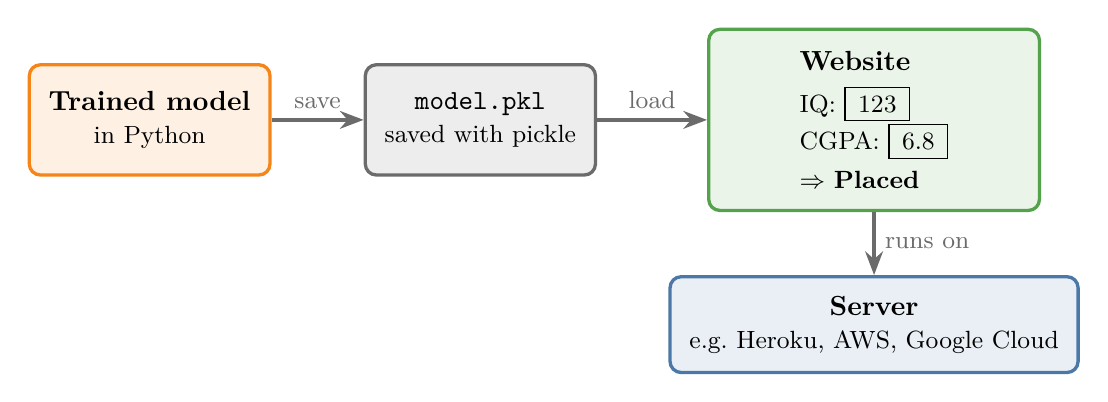
\begin{tikzpicture}
  \node[box=corange, minimum width=2.8cm, minimum height=1.4cm] (m) at (0,0) {\textbf{Trained model}\\{\small in Python}};
  \node[box=cgrey, minimum width=2.8cm, minimum height=1.4cm] (f) at (4.2,0) {\texttt{model.pkl}\\{\small saved with pickle}};
  \node[box=cgreen, minimum width=4.2cm, minimum height=2.3cm, align=left] (w) at (9.2,0)
    {\textbf{Website}\\[3pt]{\small IQ: \fbox{\,123\,}}\\{\small CGPA: \fbox{\,6.8\,}}\\[2pt]{\small $\Rightarrow$ \textbf{Placed}}};
  \node[box=cblue, minimum width=4.2cm, minimum height=1.2cm] (s) at (9.2,-2.6) {\textbf{Server}\\{\small e.g.\ Heroku, AWS, Google Cloud}};
  \draw[arrow] (m) -- node[note, above] {save} (f);
  \draw[arrow] (f) -- node[note, above] {load} (w);
  \draw[arrow] (w) -- node[note, right] {runs on} (s);
\end{tikzpicture}
\end{document}
